\documentclass{amsart}
%DIF LATEXDIFF DIFFERENCE FILE
%DIF DEL report1.tex   Sun Apr 25 19:29:39 2021
%DIF ADD report2.tex   Sun Apr 25 19:21:00 2021
\synctex=1

%=================================================================
% 
\newcount\DraftStatus  % 0 suppresses notes to selves in text
\DraftStatus=1   % TODO: set to 0 for final version
%=================================================================

%=================================================================
\usepackage{comment}
%=================================================================
%
\includecomment{JournalOnly}  
\includecomment{ConferenceOnly}  
\includecomment{TulipStyle}
%
%=================================================================
%=================================================================
% gitlatexdiff
%
%  https://gitlab.com/git-latexdiff/git-latexdiff
%=================================================================
%  git latexdiff HEAD  HEAD~5 --main templatex.tex
%  git latexdiff HEAD~1  --main templatex.tex
%  View pdf to see difference
%
%=================================================================
%
% Todo Notes for marginal comments
% 
%\newcount\DraftStatus  % 0 suppresses notes to selves in text
%\DraftStatus=1   % TODO: set to 0 for final version
\ifnum\DraftStatus=1
	\usepackage[draft,colorinlistoftodos,color=orange!30]{todonotes}
\else
	\usepackage[disable,colorinlistoftodos,color=blue!30]{todonotes}
\fi 
%\usepackage[disable]{todonotes} % notes not showed
%\usepackage[draft]{todonotes}   % notes showed
%
\makeatletter
 \providecommand\@dotsep{5}
 \def\listtodoname{List of Todos}
 \def\listoftodos{\@starttoc{tdo}\listtodoname}
 \makeatother
%
%=================================================================
%
\usepackage{color}
\newcommand{\draftnote}[3]{ 
	\todo[author=#2,color=#1!30,size=\footnotesize]{\textsf{#3}}	}
% TODO: add yourself here:
%
\newcommand{\gangli}[1]{\draftnote{blue}{GLi:}{#1}}
\newcommand{\qwu}[1]{\draftnote{red}{QWu:}{#1}}
\newcommand{\gliMarker}
	{\todo[author=GLi,size=\tiny,inline,color=blue!40]
	{Gang Li has worked up to here.}}
\newcommand{\qwuMarker}
	{\todo[author=QWu,size=\tiny,inline,color=red!40]
	{Qiong Wu has worked up to here.}}
%=================================================================

%=================================================================
%
% general packages
%  https://en.wikibooks.org/wiki/Category:Book:LaTeX
%  https://en.wikibooks.org/wiki/LaTeX/Package_Reference
%
%=================================================================
\usepackage{graphicx}
\usepackage{algorithm}
\usepackage{algorithmic}
\usepackage{breqn}
\usepackage{subcaption}
\usepackage{multirow}
\usepackage{psfrag}
\usepackage{url}
\usepackage{hyperref}
%\usepackage[colorlinks]{hyperref}
%\usepackage{cite}
\usepackage{cleveref}
\usepackage{booktabs}
\usepackage{rotating}
\usepackage{colortbl}
\usepackage{paralist}
%\usepackage{geometry}
\usepackage{epstopdf}
\usepackage{nag}
\usepackage{microtype}
\usepackage{siunitx}
\usepackage{nicefrac}
\usepackage{breakurl}
\usepackage{fontawesome}
\usepackage{xcolor}
\usepackage{multicol}
\usepackage{wrapfig}
\usepackage{todonotes}
\usepackage{tablefootnote}
\usepackage{threeparttable}
% for random text
\usepackage{lipsum}
\usepackage[english]{babel}
\usepackage[pangram]{blindtext}
% for tikz figures
\usepackage{tikz}
\usetikzlibrary{fit,positioning,arrows.meta,shapes,arrows}
%\tikzset{neuron/.style={circle,thick,fill=black!25,minimum size=17pt,inner sep=0pt},
%	input neuron/.style={neuron, draw,thick, fill=gray!30},
%	hidden neuron/.style={neuron,fill=white,draw},
%	hoz/.style={rotate=-90}}
%
%=================================================================



\begin{TulipStyle}
\usepackage[numbers]{natbib}
%=================================================================
%
% Version control information
%
%=================================================================
\usepackage{gitinfo2}
%=================================================================
\usepackage{fancyhdr}
\pagestyle{fancy}
\fancyhead{} % clear all header fields
\fancyhead[RO,LE]{\textsl{\rightmark}}
\fancyhead[LO,RE]{\ensuremath{\Rightarrow}
		\textbf{\textbf{[CONFIDENTIAL]}}\ensuremath{\Leftarrow}}
\fancyhead[CO,CE]{}
%=================================================================
\fancyfoot{} % clear all footer fields
\fancyfoot[CE,CO]{\textbf{\thepage}} 
\fancyfoot[LO,LE]{
\includegraphics[height=.9\headheight]{logos/tulip-logo.eps}
		\gitVtagn-\gitBranch\ (\gitCommitterDate)}
\fancyfoot[RO,RE]{Committed by: \textsl{\gitCommitterName}}

\setlength{\headheight}{12pt}
\renewcommand{\headrulewidth}{0.4pt}
\renewcommand{\footrulewidth}{0.4pt}
%=================================================================


%=================================================================
% for math notations
% ----------------------------------------------------------------
\usepackage{mathtools}
\usepackage{amsthm}
%
% THEOREMS -------------------------------------------------------
%
\newtheorem{thm}{Theorem}[section]
\newtheorem{cor}[thm]{Corollary}
\newtheorem{lem}[thm]{Lemma}
\newtheorem{prop}[thm]{Proposition}
\theoremstyle{definition}
\newtheorem{defn}[thm]{Definition}
\theoremstyle{remark}
\newtheorem{rem}[thm]{Remark}
\numberwithin{equation}{section}
% MATH -----------------------------------------------------------
\newcommand{\norm}[1]{\left\Vert#1\right\Vert}
\newcommand{\abs}[1]{\left\vert#1\right\vert}
\newcommand{\set}[1]{\left\{#1\right\}}
\newcommand{\Real}{\mathbb R}
\newcommand{\eps}{\varepsilon}
\newcommand{\To}{\longrightarrow}
\newcommand{\BX}{\mathbf{B}(X)}
% ----------------------------------------------------------------
\newcommand{\I}{{\cal I}}
\newcommand{\Id}{{\cal I} }
\newcommand{\Dc}{{\cal D}}
\newcommand{\J}{{\cal J}}
\newcommand{\Dn}{{\cal D}_n}
\newcommand{\Dd}{{\cal D}_n }
\renewcommand{\P}{{\cal P}}
\newcommand{\Nu}{{\cal N} }
\newcommand{\B}{{\cal B}}
\newcommand{\Bf}{{\bf B}}
\newcommand{\Y}{{\bf Y}}
\newcommand{\A}{{\cal A}}
% ----------------------------------------------------------------
\newcommand{\V}{{\cal V}}
\newcommand{\M}{{\cal M}}
\newcommand{\F}{{\cal F}}
\newcommand{\Fd}{{\cal F}}
\newcommand{\BF}{{\cal BF}_n}
\newcommand{\BFd}{{\cal BF}_n}
\newcommand{\TF}{{\cal TF}_n}
\newcommand{\TFd}{{\cal TF}_n}
%\newcommand{\G}{{\cal G}}
\newcommand{\X}{{\cal X}}
\newcommand{\E}{{\cal E}}
\newcommand{\K}{{\cal K}}
\newcommand{\T}{{\cal T}_n}
\renewcommand{\H}{{\cal H}}
% ----------------------------------------------------------------
\newtheorem{Remark}{Remark}
\newtheorem{proposition}{Proposition}
\newtheorem{theorem}{Theorem}
\newtheorem{lemma}{Lemma}
\newtheorem{corollary}{Corollary}
\newtheorem{example}{Example}
\newtheorem{definition}{Definition}
\newtheorem{Algorithms}{Algorithm}
% ----------------------------------------------------------------
\newcommand{\bu}{{\mathbf 1} }
\newcommand{\bo}{{\mathbf 0} }
\newcommand{\N}{\mbox{{\sl l}}\!\mbox{{\sl N}}}
% ----------------------------------------------------------------
\def\uint{[0,1]}
\def\proof{{\scshape Proof}. \ignorespaces}
\def\endproof{{\hfill \vbox{\hrule\hbox{%
   \vrule height1.3ex\hskip1.0ex\vrule}\hrule
  }}\par}
%
%=================================================================

\hypersetup
{
    pdfauthor={\gitAuthorName},
    pdfsubject={TULIP Lab},
    pdftitle={},
    pdfkeywords={TULIP Lab, Data Science},
%	bookmarks=true,  
}

\end{TulipStyle}




%=================================================================
%
%DIF PREAMBLE EXTENSION ADDED BY LATEXDIFF
%DIF UNDERLINE PREAMBLE %DIF PREAMBLE
\RequirePackage[normalem]{ulem} %DIF PREAMBLE
\RequirePackage{color}\definecolor{RED}{rgb}{1,0,0}\definecolor{BLUE}{rgb}{0,0,1} %DIF PREAMBLE
\providecommand{\DIFadd}[1]{{\protect\color{blue}\uwave{#1}}} %DIF PREAMBLE
\providecommand{\DIFdel}[1]{{\protect\color{red}\sout{#1}}}                      %DIF PREAMBLE
%DIF SAFE PREAMBLE %DIF PREAMBLE
\providecommand{\DIFaddbegin}{} %DIF PREAMBLE
\providecommand{\DIFaddend}{} %DIF PREAMBLE
\providecommand{\DIFdelbegin}{} %DIF PREAMBLE
\providecommand{\DIFdelend}{} %DIF PREAMBLE
\providecommand{\DIFmodbegin}{} %DIF PREAMBLE
\providecommand{\DIFmodend}{} %DIF PREAMBLE
%DIF FLOATSAFE PREAMBLE %DIF PREAMBLE
\providecommand{\DIFaddFL}[1]{\DIFadd{#1}} %DIF PREAMBLE
\providecommand{\DIFdelFL}[1]{\DIFdel{#1}} %DIF PREAMBLE
\providecommand{\DIFaddbeginFL}{} %DIF PREAMBLE
\providecommand{\DIFaddendFL}{} %DIF PREAMBLE
\providecommand{\DIFdelbeginFL}{} %DIF PREAMBLE
\providecommand{\DIFdelendFL}{} %DIF PREAMBLE
%DIF LISTINGS PREAMBLE %DIF PREAMBLE
\RequirePackage{listings} %DIF PREAMBLE
\RequirePackage{color} %DIF PREAMBLE
\lstdefinelanguage{DIFcode}{ %DIF PREAMBLE
%DIF DIFCODE_UNDERLINE %DIF PREAMBLE
  moredelim=[il][\color{red}\sout]{\%DIF\ <\ }, %DIF PREAMBLE
  moredelim=[il][\color{blue}\uwave]{\%DIF\ >\ } %DIF PREAMBLE
} %DIF PREAMBLE
\lstdefinestyle{DIFverbatimstyle}{ %DIF PREAMBLE
	language=DIFcode, %DIF PREAMBLE
	basicstyle=\ttfamily, %DIF PREAMBLE
	columns=fullflexible, %DIF PREAMBLE
	keepspaces=true %DIF PREAMBLE
} %DIF PREAMBLE
\lstnewenvironment{DIFverbatim}{\lstset{style=DIFverbatimstyle}}{} %DIF PREAMBLE
\lstnewenvironment{DIFverbatim*}{\lstset{style=DIFverbatimstyle,showspaces=true}}{} %DIF PREAMBLE
%DIF END PREAMBLE EXTENSION ADDED BY LATEXDIFF

\begin{document}
%
%=================================================================
%
\title[Report]{FILP 00 Final Report}%

\author{Mingxi Wang}
\address[A.~1]{School of Computer Science,\\ 
Jilin University, ChangChun 130012, China}%
\email[A.~1]{mxwang@tulip.academy}


%\thanks{Thanks to \ldots}%
\subjclass{Artificial Intelligence}%
\date{\gitAuthorDate}%


\begin{abstract}
In this report, I will talk about my work achievements, including the learning and practice of GIT uploading, downloading and remote connection, as well as the topic selection and programming practice of Kaggle
\end{abstract}

\keywords{}%




\maketitle
\tableofcontents

\newpage
%=================================================================

%wmxgaidongde
%%=================================================================
\section{Introduction}\label{sec-intro}

\section{Preliminaries} \label{sec-preliminaries}

\section{Method} \label{sec-method}

\section{Experiment and Analysis} \label{sec-experiment}

\section{Conclusions} \label{sec-conclusions}

\section*{Acknowledgement}

%\lipsum[1]


The authors would like to thank \ldots


\section{Research motivation and context}



\subsection{\DIFdelbegin \DIFdel{Work target}\DIFdelend \DIFaddbegin \DIFadd{Project Objectives}\DIFaddend }
The project analyzed 12 years of crime reports from all of San Francisco's neighborhoods to create a model that can predict crime categories at a given time and place.\\

\subsection{Project background}
Crime is a kind of behavior that does great harm to the society. \DIFaddbegin \DIFadd{It brings great loss of life and property to human beings.}\DIFaddend In modern society, human beings \DIFdelbegin \DIFdel{always prevent crime by making }\DIFdelend \DIFaddbegin \DIFadd{prevent crime through }\DIFaddend strict judicial means, and research on crime prevention based on sociology, psychology and law.\\

%wmx:\hspace*{0.6cm} is The indentation symbol
\hspace*{0.6cm}The objective of this project is to quantitatively analyze a data set of nearly 12 years of crime reports \DIFaddbegin \DIFadd{from all San Francisco neighborhoods }\DIFaddend by computer means and to create a model that predicts the type of crime that will occur given information such as time and location.\DIFdelbegin \DIFdel{The number of crime types is fixed, and our model is essentially a processor for a multi-classification problem}\DIFdelend \\


\newpage
\section{Research contents and methods}

\subsection{Evaluation metric}
	\begin{itemize}
		\item 878,049 samples, a total of 9 features.
	\end{itemize}
	\begin{itemize}
	\item Date, category, description, day of the week, name of the police district, solution, approximate street address of the crime, longitude, latitude.
	\end{itemize}

	.\\

	\begin{itemize}
	\item First date:  2003-01-06 00:01:00
	\end{itemize}
	\begin{itemize}
	\item Last date:  2015-05-13 23:53:00
	\end{itemize}
	\begin{itemize}
	\item Test data shape  (878049, 9)
	\end{itemize}

	
	\begin{center}
		\begin{figure}[htbp]
			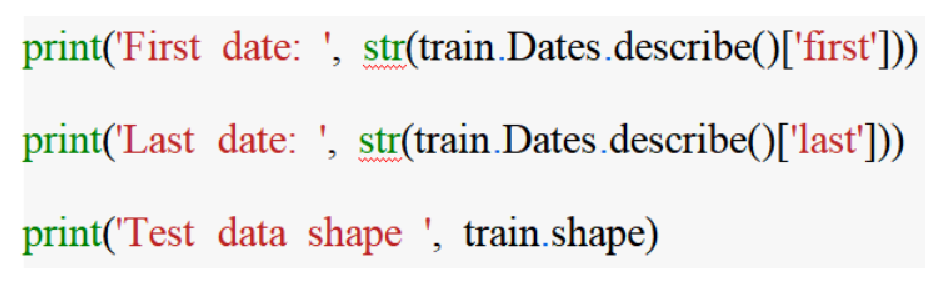
\includegraphics[scale=0.6]{./pic/qmcode1.eps}
			\caption{preview I}
		\end{figure}
	\end{center}

	\begin{center}
	\begin{figure}[htbp]
		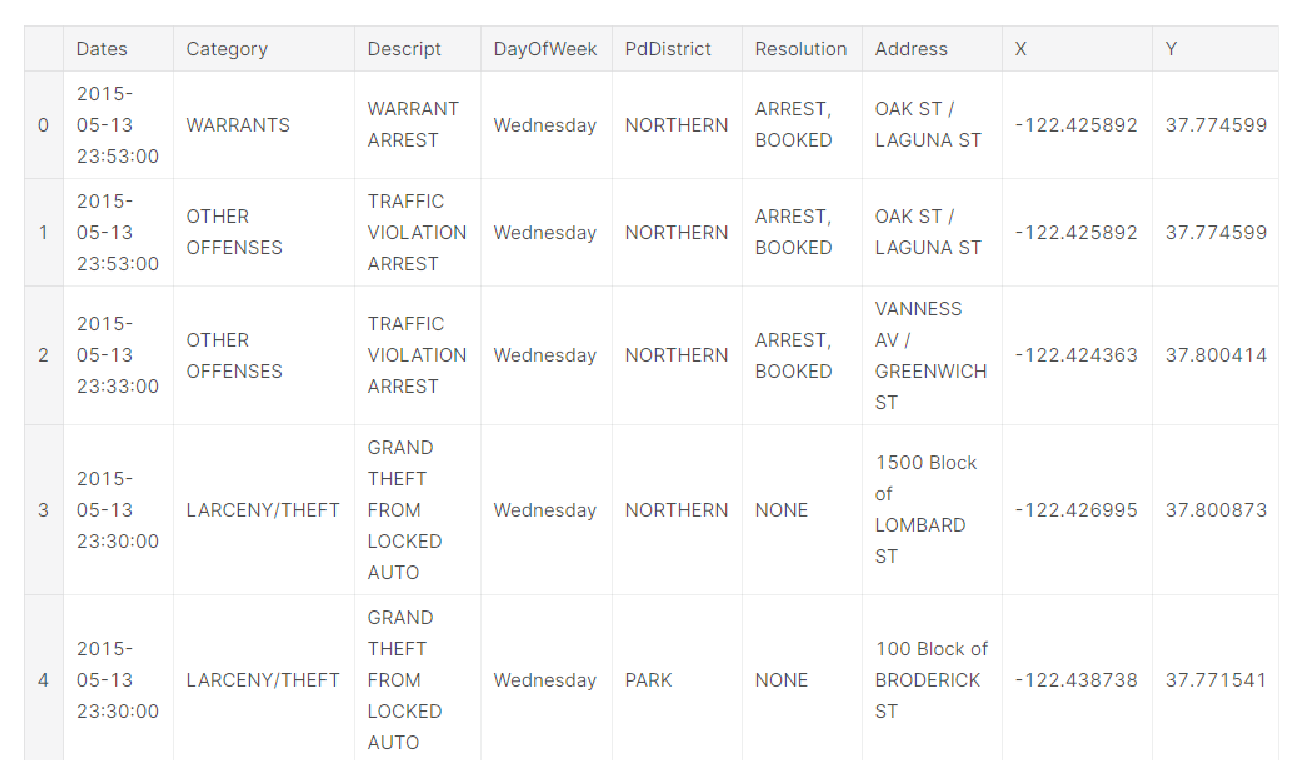
\includegraphics[scale=0.5]{./pic/qmyangben.eps}
		\caption{preview II}
	\end{figure}
\end{center}

\newpage

\subsection{Data cleaning}
	\begin{itemize}
		\item There are 2323 duplicate items that need to be removed
	\end{itemize}
	train.duplicated().sum()
	\begin{itemize}
		\item Throw away samples in a range of longitude and latitude (e.g., 50)
	\end{itemize}

\subsection{Characteristics of the engineering}
	\begin{center}
		\begin{figure}[htbp]
			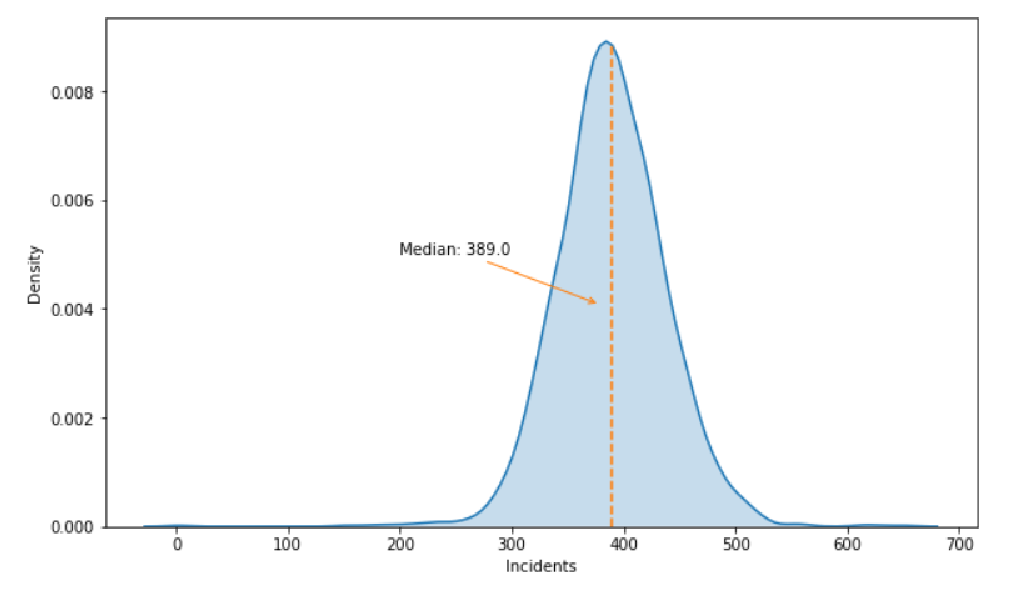
\includegraphics[scale=0.7]{./pic/qmzhengtai.eps}
			\caption{Distribution of number of incidents per day}
		\end{figure}
	\end{center}
\hspace*{0.6cm}Similarly, there was no significant deviation in the frequency of events over the course of the week.
\begin{center}
	\begin{figure}[htbp]
		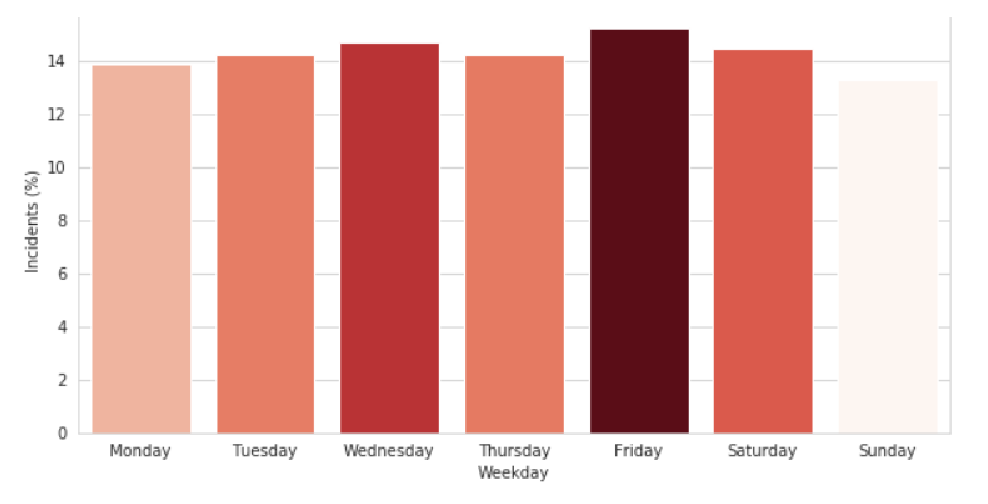
\includegraphics[scale=0.7]{./pic/qmzhifangtu.eps}
		\caption{incidents per Weekday}
	\end{figure}
\end{center}
\hspace*{0.6cm}A total of 39 discrete categories of incidents were recorded by police stations, the most common being theft (19.91\%), non-criminal cases (10.50\%) and assault (8.77\%)

\begin{figure}[htbp]
	\includegraphics[scale=0.5]{./pic/qmshuxingtu.eps}
	\caption{incidents per Crime Category}
\end{figure}

	\hspace*{0.6cm}The chart below shows the average number of incidents per hour for the five crime categories.
	\DIFdelbegin \DIFdel{Different }\DIFdelend \DIFaddbegin \DIFadd{Obviously, different }\DIFaddend crimes occur with different frequencies \DIFdelbegin \DIFdel{, depending on the time of day
	}\DIFdelend \DIFaddbegin \DIFadd{at different times of the day.
	}\DIFaddend Prostitution, for example, takes place mostly at night, gambling incidents take place from late at night until morning, and burglaries from early morning until afternoon.
	As before, this is clear evidence that time parameters will also play an important role.

	\begin{figure}[htbp]
		\includegraphics[scale=0.7]{./pic/qmzhexiantu.eps}
		\caption{average number of incidents per hour}
	\end{figure}

	\begin{itemize}
	\item From the "Date" field, we extracted the \DIFdelbegin \DIFdel{Date}\DIFdelend \DIFaddbegin \DIFadd{date}\DIFaddend , month, year, \DIFdelbegin \DIFdel{hour, and minute}\DIFdelend \DIFaddbegin \DIFadd{hours, minutes, days, and days since the first day}\DIFaddend .
	\item We \DIFdelbegin \DIFdel{extract the location of the event }\DIFdelend \DIFaddbegin \DIFadd{extracted }\DIFaddend from the "Address" field \DIFdelbegin \DIFdel{, and we can tell whether it happened }\DIFdelend \DIFaddbegin \DIFadd{whether the event occurred }\DIFaddend at the intersection or \DIFdelbegin \DIFdel{inside the building }\DIFdelend \DIFaddbegin \DIFadd{on a building component}\DIFaddend .
\end{itemize}

\subsection{Information coding}
	The discrete data is converted to a number between 0 and N-1, where N is the number of different values in a list.You can think of it as the number of different values of a feature.\\

\subsection{Training model}
	\begin{itemize}
		\item Train 23 Epochs.
		\item Use cross validation to evaluate the quality of our model.\\
		After training, the model obtained:
		\item a cross validation score of 2.46.
		\item it got 2.49 on the test set.
	\end{itemize}



\newpage

\section{Architecture of the model}

The model architecture consists of six steps, as follows:\\

	\begin{itemize}
	\item 1. Make the decision tree fit the data\\
	\item 2. Evaluation model\\
	\item 3. Add weight to incorrect samples.\\
	\item 4. Select the leaf nodes with the greatest incremental loss for growth.\\
	\item 5. Generate the tree at the node in the previous step.\\
	\item 6. Go to Step 2 for the cycle\\
\end{itemize}

\newpage
\section{Conclusion}

	Conclusion: \DIFdelbegin \DIFdel{Our }\DIFdelend \DIFaddbegin \DIFadd{Based on data analysis, processing and utilization, our }\DIFaddend model can effectively predict \DIFdelbegin \DIFdel{some types of crime .In addition, by }\DIFdelend \DIFaddbegin \DIFadd{crime types.By }\DIFaddend using the multi-classification algorithm to analyze the input features and update the model parameters \DIFaddbegin \DIFadd{through iterative training}\DIFaddend , our model \DIFdelbegin \DIFdel{gets }\DIFdelend \DIFaddbegin \DIFadd{can be trained }\DIFaddend more and more \DIFdelbegin \DIFdel{accurate training.In order }\DIFdelend \DIFaddbegin \DIFadd{accurately.So as }\DIFaddend to complete the task of classification prediction.\\
	\\


% ----------------------------------------------------------------
%\newpage
%\bibliography{tuliplab,yourbib}
% TODO: you should change this yourbib into a proper bib file name
%\bibliographystyle{plainnat}
%=================================================================

%\listoftodos

\end{document}

